\section{Methods}  \label{Methods}

This section details the methodologies employed in the current research. It starts with an introduction to novel recurrent perceiver architectures—specifically the Recurrent Perceiver (RPerceiver) and its multi-modal extension, the RPerceiverMM—which are engineered to process high-dimensional temporal data, such as video sequences, for object detection tasks. The subsequent section discusses the custom-generated "detection-moving-mnist-easy" dataset, developed to facilitate the evaluation of model capabilities in video object detection and center point localization. Following this, training procedures are described, including dropout and shuffle techniques, implemented to enhance model robustness against sensor unreliability and non-deterministic input sequences. The section then elaborates on the adopted loss function for the set prediction problem. Finally, performance evaluation metrics are outlined, including Mean Average Precision (mAP) for object detection, and Average Displacement Error (ADE) and Final Displacement Error (FDE) for the center point prediction task.

\subsection{Model} \label{Methods:Model}

A new Recurrent Perceiver (RPerceiver) is introduced, a Recurrent Neural Network (RNN) capable of processing high-dimensional inputs. This architecture draws inspiration from the Perceiver \cite{jaeglePerceiverGeneralPerception2021}, noted for its ability to handle high-dimensional data.

The Perceiver architecture has been re-engineered by incorporating a temporal dimension, effectively unrolling it over time. This modification addresses the original Perceiver's limitation of producing only a single output per input, a characteristic that renders it unsuitable for sequence tasks with a temporal component, such as video object detection. Whereas previously the Perceiver was only unrolled in depth, the loop has now been closed, and it is unrolled in time by propagating the latent array between time steps. The architecture of the RPerceiver is illustrated in Figure \ref{fig:figure_methods_recurrent_perceiver}.

\begin{figure}
    \centering
    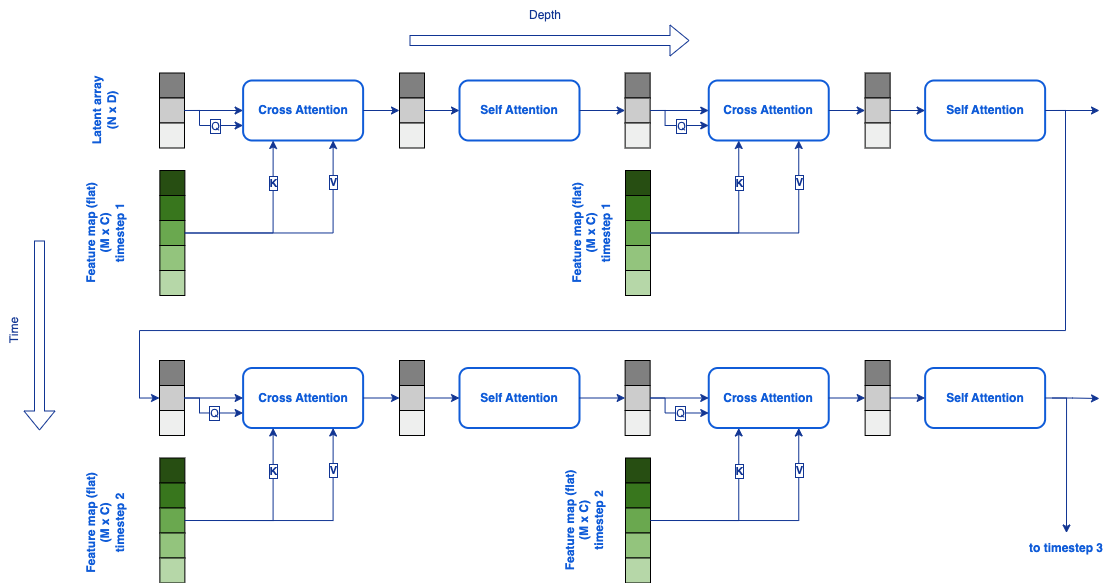
\includegraphics[width=\textwidth]{figures/figure_methods_recurrent_perceiver.png}
    \caption{The Recurrent Perceiver (RPerceiver) architecture processes inputs along the time dimension by propagating the latent array between time steps. In the depth dimension (within a single time step), this example shows two RPerceiver layers.}
    \label{fig:figure_methods_recurrent_perceiver}
\end{figure}

% TODO: Read about calibration problem.
A variation of the RPerceiver architecture capable of processing multi-modal inputs is proposed, termed the Recurrent Perceiver Multi-Modal (RPerceiverMM). The original Perceiver paper \cite{jaeglePerceiverGeneralPerception2021} addressed multi-modality by concatenating a learned, modality-specific encoding to each input element. Modern Autonomous Driving Systems (ADS) process information from multiple sensors, often incorporating multiple cameras positioned in different locations, which introduces a calibration challenge. Consequently, this work adopts a distinct approach to multi-modality. A sensor-specific cross-attention module is introduced to the RPerceiverMM. Within the scope of this thesis, the focus is on a multi-view camera setup. The architecture of the RPerceiverMM is illustrated in Figure~\ref{fig:figure_methods_recurrent_perceiver_mm}.

\begin{figure}
    \centering
    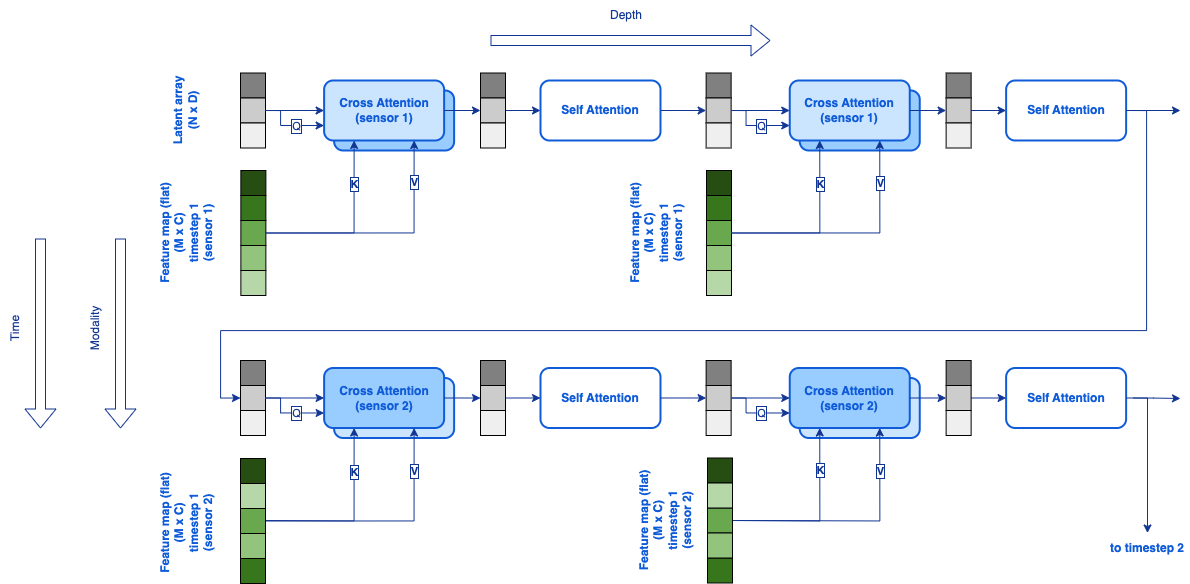
\includegraphics[width=\textwidth]{figures/figure_methods_recurrent_perceiver_mm.png}
    \caption{The Recurrent Perceiver Multi-Modal (RPerceiverMM) architecture operates along time, depth, and an additional modality dimension, designed for multi-view camera inputs. It employs camera-specific cross-attentions (shown in different colors), which have their own weights, to process information from different sensors (views). In this example, separate cross-attention blocks are used for each camera input, integrating modality-specific information.}
    \label{fig:figure_methods_recurrent_perceiver_mm}
\end{figure}

In addition to the RPerceiver module, a CNN backbone and detection heads were utilized. This backbone served to learn a $2D$ representation of the input frames. This backbone was designed with four blocks, each containing convolutional layers and ReLU activation. Each block progressively downscales spatial dimensions by a factor of $2$ while concurrently increasing channel dimensionality. This process results in a final feature map possessing $128$ channels and $\frac{1}{16}$ of the original spatial resolution.

The output features generated by the RPerceiver module are subsequently passed to the detection heads, which are tasked with predicting object labels and their corresponding positions. Detection heads identical to those employed in the DETR model \cite{carionEndtoEndObjectDetection2020} were adopted. These heads incorporate a linear layer to predict the class label via a softmax function, and a $3$-layer Multi-Layer Perceptron (MLP) featuring ReLU activation functions to predict object coordinates. Two variants for object coordinates were considered: (i) bounding boxes, wherein the MLP predicts the normalized center coordinates, height, and width relative to the input image, and (ii) center points. The respective output dimensions for these variants are $N \times 4$ and $N \times 2$, where $N$ denotes a fixed number of detection slots (queries). Given that $N$ is typically substantially larger than the actual number of objects present, a special class label, $\emptyset$, is employed to signify that no object is detected within a particular slot, thereby fulfilling a role analogous to a background class.

For bounding box predictions, a sigmoid activation function was used to predict the normalized coordinates of the bounding box center, as well as its width and height. In the case of center points, a tanh activation function was utilized. This selection was based on positioning the origin of the coordinate system at the center of the image raster, thereby emulating a bird's-eye view perspective, akin to an Autonomous Driving System (ADS) positioned centrally with comprehensive surrounding views. The complete architecture of the model is shown in Figure~\ref{fig:figure_methods_recurrent_perceiver_complete}.

\begin{figure}
    \centering
    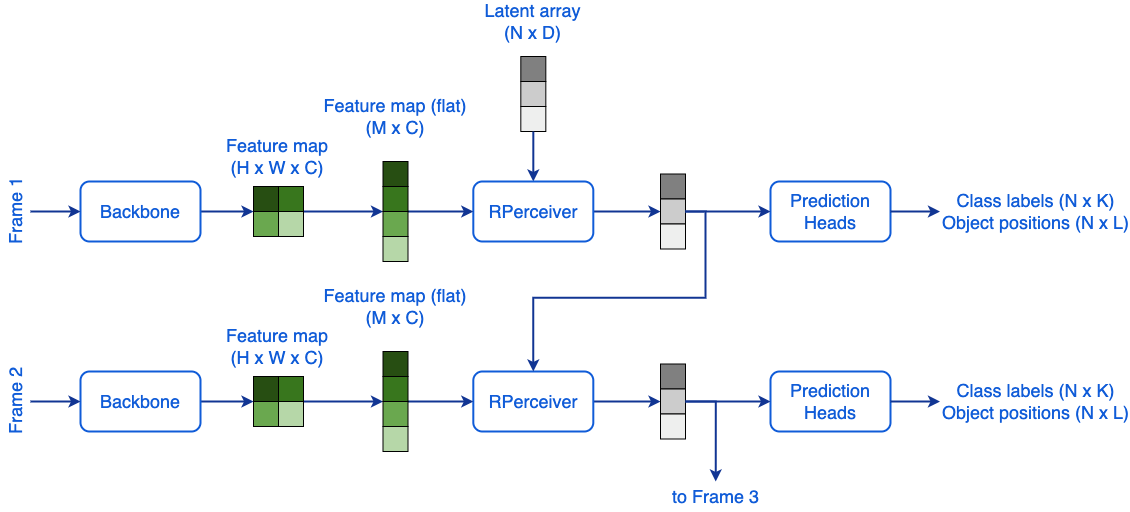
\includegraphics[width=\textwidth]{figures/figure_methods_recurrent_perceiver_complete.png}
    \caption{Full architecture of the model, including RPerceiver, Backbone, and Detection Heads. Input frames are processed by a Backbone network to extract a feature map. This flattened feature map, along with a latent array propagated from the previous time step, is fed into a Recurrent Perceiver (RPerceiver). The RPerceiver's output embedding is then used by Prediction Heads to determine class labels and object positions for the current frame.}
    \label{fig:figure_methods_recurrent_perceiver_complete}
\end{figure}

The intuition behind the RPerceiver architecture for object detection is that the variable $N$, a dimension of the latent array, represents the number of objects the RPerceiver tracks, while $D$ represents the number of attributes for each object (e.g., position, dimension, color, speed, etc.). In order to revalidate the existence of an object across different modalities by utilizing cross-attention to match its position, dimensions, and color with sensor input. Periodically, the system must initiate tracking for new objects within its $N$ available slots, necessitating a mechanism to monitor slot utilization.

\subsection{Dataset} \label{Methods:Dataset}

For this experiment, a custom dataset was generated, named "detection-moving-mnist-easy". The dataset design was inspired by the MovingMNIST dataset \cite{srivastava2016unsupervisedlearningvideorepresentations}, which is commonly used for tasks like video prediction, unsupervised feature learning from video. In this case, the focus is on video object detection and a simplified variation of keypoints, where the prediction involves the center point of the object. This task is similar to keypoint detection as the object's center point, rather than the bounding box center, is predicted. The dataset is hosted on Hugging Face Hub \footnote{\url{https://huggingface.co/datasets/Max-Ploter/detection-moving-mnist-easy}}.

For the first frame, a number of digits, ranging from $1$ to $10$, is selected with uniform probability (see Figure~\ref{fig:figure_method_dataset_train_digit_classes}). Depending on the number of digits selected for the first frame, digits are drawn, without replacement, from the well-known MNIST dataset \cite{lecunGradientbasedLearningApplied1998} (from the train and test splits corresponding to the dataset split). Each digit is placed on the first frame of the $128 \times 128$ canvas image. A greedy algorithm is employed to randomly place digits on the first frame while attempting to avoid overlaps. This initial separation is intended to simplify object detection for the model at the start of the sequence. To each digit, an affine translation ranging from $-5$ to $5$ pixels is randomly assigned with uniform probability. Then, corresponding affine transformations are applied to move the digits through $20$ frames on the $128 \times 128$ canvas image. As a result, this process yields a tensor of size $20 \times 1 \times 128 \times 128$, representing a video sequence (see Figure~\ref{fig:figure_methods_dataset_detection_mmnist_sequence}).

\begin{figure}
    \centering
    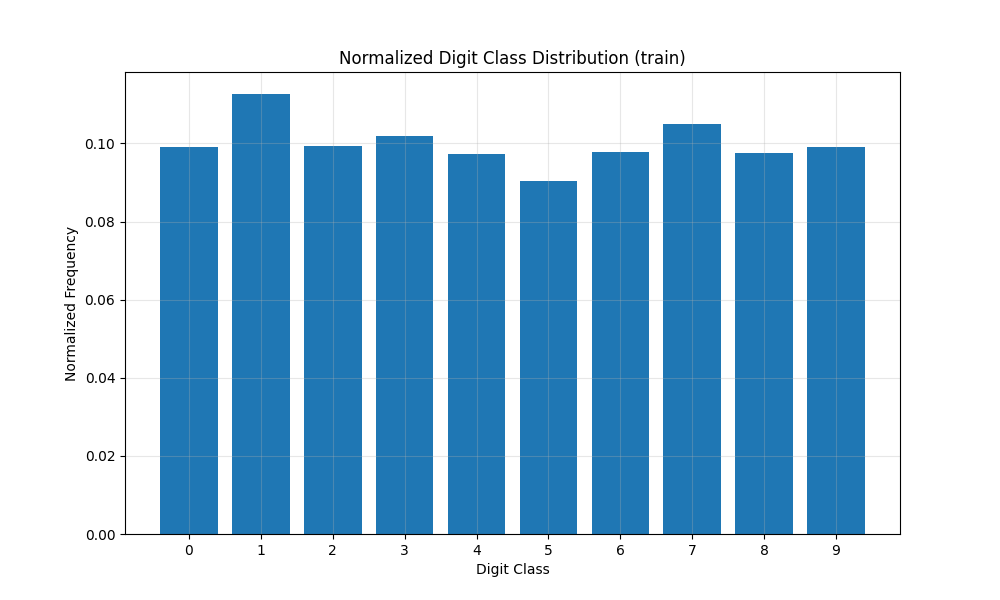
\includegraphics[width=\textwidth]{figures/figure_method_dataset_train_digit_classes.png}
    \caption{Distribution of classes in the "detection-moving-mnist-easy" dataset.}
    \label{fig:figure_method_dataset_train_digit_classes}
\end{figure}

To make the dataset more challenging, digit overlap is not restricted in subsequent frames. Some degree of overlap in the first frame is possible if the greedy algorithm is unable to randomly place all digits without overlap. Digits are not bounced against image boundaries, allowing each digit to potentially leave the frame. As illustrated in Figure~\ref{fig:figure_method_dataset_train_digits_per_frame}, later frames may contain fewer digits.

\begin{figure}
    \centering
    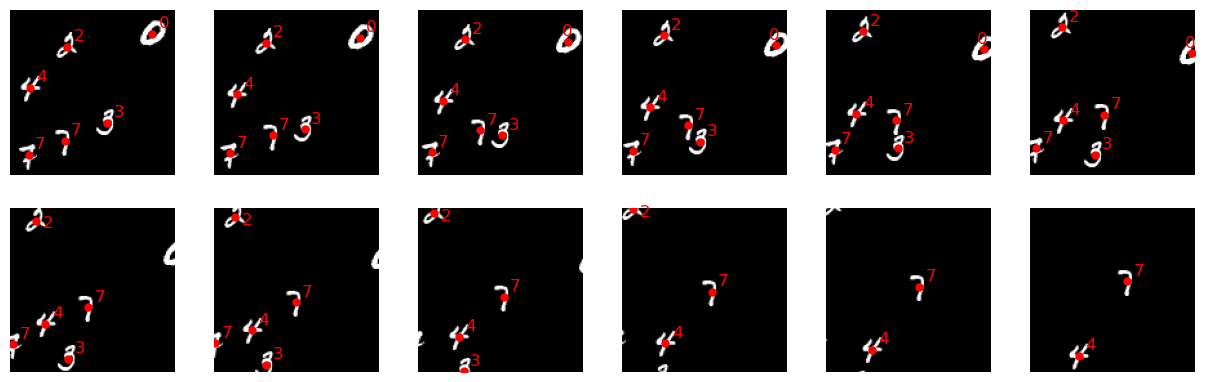
\includegraphics[width=\textwidth]{figures/figure_methods_dataset_detection_mmnist_sequence.png}
    \caption{Example of 12 frames from the sequence. Ground truth, shown in red, indicates the ground truth digit center point and a class label.}
    \label{fig:figure_methods_dataset_detection_mmnist_sequence}
\end{figure}

% TODO DOUBLE CHECK number this plot
\begin{figure}
    \centering
    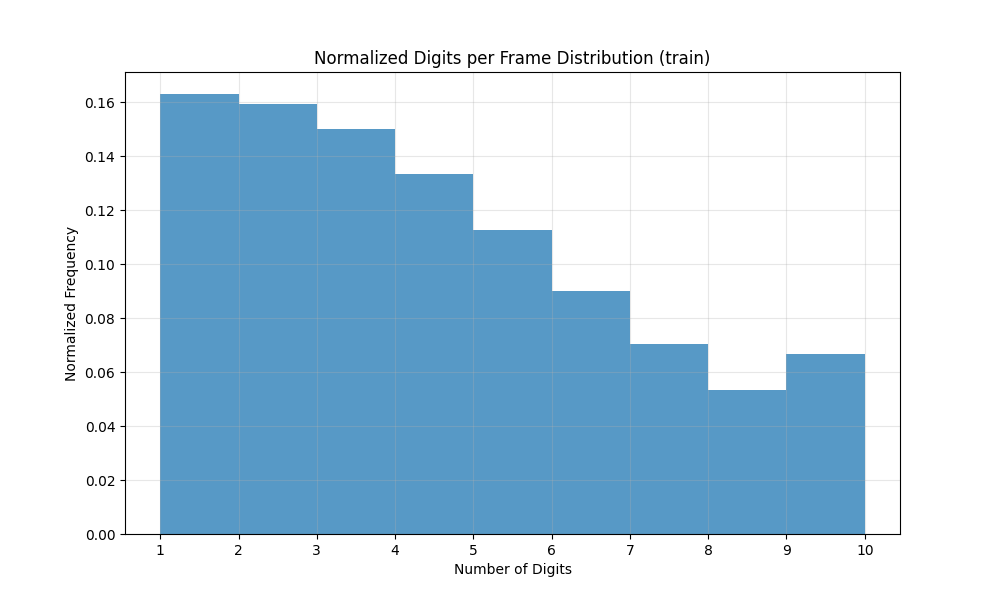
\includegraphics[width=\textwidth]{figures/figure_method_dataset_train_digits_per_frame.png}
    \caption{Normalized frequency distribution of the number of digits per frame for the \textbf{train split} of the "detection-moving-mnist-easy" dataset. The histogram illustrates that frames containing a smaller number of digits (notably 1 to 3) are observed with the highest normalized frequency. This distribution, skewed towards fewer digits per frame, is a characteristic outcome of the dataset's generation process where digits can move and exit the frame boundaries over time, as their movement is not confined within the frame.}
    \label{fig:figure_method_dataset_train_digits_per_frame}
\end{figure}

The dataset was generated with $60,000$ training samples and $10,000$ testing samples. Annotations, automatically generated during sequence creation, include digit classes, digit center point coordinates (keypoints), bounding box coordinates, and digit identity IDs.

\subsection{Dropout and Shuffle} \label{Methods:DropoutAndShuffle}

As previously discussed in Section~\ref{Background:AutonomousDrivingSystems}, Autonomous Driving Systems (ADSs) face challenges related to sensor reliability. Two critical identified issues are the potential for complete sensor failure, where a sensor modality ceases to provide any data, and the non-deterministic availability of sensor inputs. To enhance the resilience of perception models against these real-world imperfections, this work investigates training strategies designed to improve model robustness. Specifically, the aim is to experimentally evaluate how models perform when subjected to simulated conditions mimicking both complete sensor data loss (akin to sensor failure) and non-deterministic input sequences (akin to middleware-induced timing variations). The following training procedures, \texttt{dropout} and \texttt{shuffle}, are introduced to directly address these challenges during the model training phase. A model trained without applying these training procedures is considered the baseline.

\begin{description}
    \item[\texttt{shuffle}] In this procedure, the sensor inputs are randomly permuted within each time step. Consequently, the model receives inputs from the sensors in a random order for that specific time step. This shuffling only occurs for sensor inputs within the same time step and aims to simulate the non-deterministic ordering of inputs that can occur due to middleware asynchronicity. This training procedure is therefore relevant for models that process data from multiple distinct sensors at each time step.    
    \item[\texttt{dropout}] This procedure simulates scenarios where sensor information is missing, directly addressing the challenge of potential complete sensor failure for one or more modalities. To achieve this, the model is trained by intermittently dropping sensor inputs (input dropout). The first half of the input sequence is kept intact (no dropout), allowing the model to accumulate features in its hidden state. The second half of the sequence may undergo frame dropout depending on the dropout probability. During training, the probability of an information dropout is gradually increased from 10\% up to 86.6\%.
\end{description}

The \texttt{dropout} procedure is shown in Figure~\ref{fig:figure_methods_recurrent_perceiver_with_dropout}. The pseudo code is shown in Appendix~\ref{Appendix:TrainProcedures}.

\begin{figure}
    \centering
    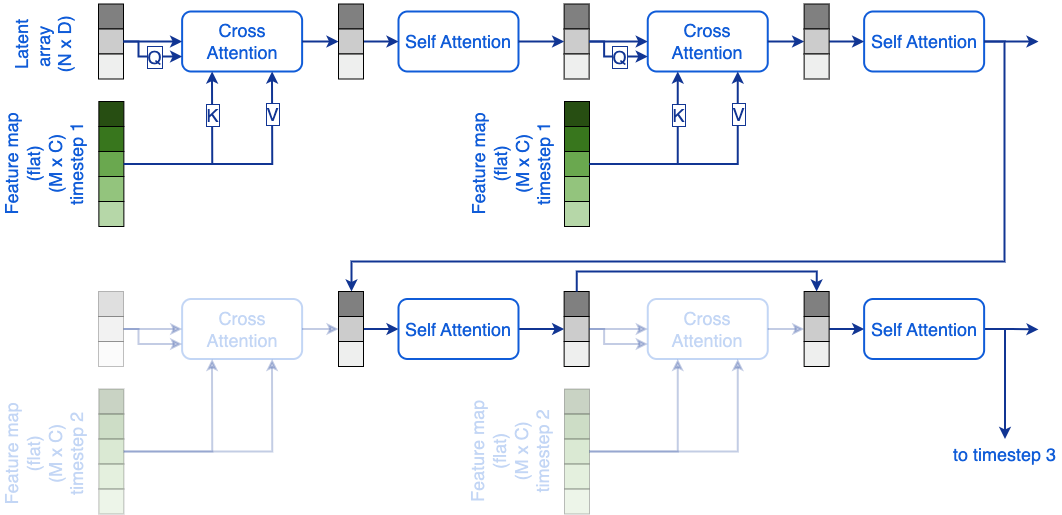
\includegraphics[width=\textwidth]{figures/figure_methods_recurrent_perceiver_with_dropout.png}
    \caption{Diagram of the \texttt{dropout} mechanism in action. Timestep 1 shows normal operation where the input feature map is processed by the backbone (implied before cross-attention) and then fused with the latent array via cross-attention, followed by self-attention. Timestep 2 illustrates a dropout event: the input feature map and the cross-attention block are shown faded, indicating that this sensor view's data is dropped. Consequently, the cross-attention step, which incorporates new sensor information (K, V), is skipped. However, the latent array is still updated by the self-attention mechanism, demonstrating the model's reliance on its internal memory when an input is missing. Intuitively, this self-attention acts like a 'propagate forward' step in a tracker: it updates the object's presumed state based on prior motion even without current sensor input. This internal prediction maintains continuity and can be corrected by cross-attention when new sensor data becomes available and is processed.}
    \label{fig:figure_methods_recurrent_perceiver_with_dropout}
\end{figure}

\subsection{Loss Function} \label{Methods:LossFunction}

The loss calculation approach was adopted from \cite{carionEndtoEndObjectDetection2020, stewartEndtoendPeopleDetection2015}. The proposed model in the Section~\ref{Methods:Model} predicts a fixed-size set of $N$ potential objects per timestep. The parameter $N$ is a dimension of the latent array and is chosen to be greater than the cardinality of the largest set of ground-truth objects per frame. The model uses an attention mechanism that allows it to attend to all other elements in the attention map. Therefore, there is no predefined structure, like a grid in one-stage image detectors \cite{redmonYouOnlyLook2016}, associating predictions with ground-truth objects. This presents the core challenge of how to score the fixed-size prediction set against the variable-size ground-truth set. The loss function calculation consists of two steps: first, finding an optimal bipartite matching between the elements of the predicted and ground-truth sets, and second, calculating a loss.

Let us denote the set of predictions for a given timestep as $ \hat{Y} = \{\hat{y}_j\}_{j=1}^N $ and the corresponding set of ground-truth objects for that frame as $ Y = \{y_i\}_{i=1}^M $ where $ N > M $. At each recurrence (i.e., for each frame/timestep processed), the RPerceiver outputs the entire set of $N$ predictions $\hat{Y}$. Each prediction $\hat{y}_j \in \hat{Y}$ consists of a predicted object position $\hat{o}_j$ and a predicted class label $\hat{c}_j$ (including the possibility of the no-object class $\emptyset$). The position $\hat{o}_j$ can represent different objects depending on the specific task:
\begin{itemize}
    \item For the \textbf{bounding box prediction task}, $\hat{o}_j$ is the predicted box $\hat{b}_j = (\hat{b}_x, \hat{b}_y, \hat{b}_w, \hat{b}_h) \in \mathbb{R}^4$, representing center coordinates, height, and width relative to the frame size.
    \item For the \textbf{center point prediction task}, $\hat{o}_j$ is the predicted center point coordinates $\hat{p}_j = (\hat{p}_x, \hat{p}_y) \in \mathbb{R}^2$ relative to the frame size.
\end{itemize}
Similarly, each ground-truth object $y_i \in Y$ consists of the ground-truth object position $o_i$ (either a box $b_i$ or a point $p_i$) and the ground-truth class label $c_i$.
A matching algorithm is defined via an injective function $f: Y \rightarrow \hat{Y}$, where $f(y_i)$ is the candidate hypothesis $\hat{y}_j \in \hat{Y}$ assigned to the ground-truth object $y_i$. Given $f$, a loss function on pairs of sets $Y$ and $\hat{Y}$ is defined as \cite{stewartEndtoendPeopleDetection2015}:

\begin{equation} \label{eq:set_loss}
\mathcal{L}(Y, \hat{Y}, f ) = \sum_{i=1}^{M} \mathcal{L}_{pos}(y_i, f(y_i)) +  \sum_{j=1}^{N} \mathcal{L}_c (\hat{y}_j, f^{-1}(\hat{y}_j))
\end{equation}

where $\mathcal{L}_{pos}$ is the object localization loss. The specific formulation of $\mathcal{L}_{pos}$ depends on the task (bounding box or center point). $\mathcal{L}_c$ is the class prediction loss, for which the Focal Loss was used \cite{linFocalLossDense2018}. $f^{-1}(\cdot)$ is an inverse of the matching function $f$:

\begin{equation*}
f^{-1}(\hat{y}_j) =
\begin{cases}
y_i & \exists \, y_i \in Y, f(y_i) = \hat{y}_j \\
\emptyset & \text{otherwise} \\
\end{cases}
\end{equation*}
Details on each loss term are provided below.

% TODO Mention hyperparameters
\textbf{Focal Loss.} The Focal Loss \cite{linFocalLossDense2018} is used to address the class imbalance between the foreground objects and the numerous potential background predictions. The class loss component $\mathcal{L}_c$ for each prediction $\hat{y}_j$ involves the sigmoid Focal Loss. The total class loss for a prediction $\hat{y}_j$ is summed over all foreground classes $k \in \{1, ..., C\}$, where $C$ is the number of object categories (excluding the $\emptyset$ class). The Focal Loss for a single class $k$ and prediction $j$ is defined using the $\alpha$-balanced form:
\begin{equation} \label{eq:focal_loss_corrected}
    \text{FL}(p_{jk}, y_{jk}) = - \alpha_t (1 - p_t)^\gamma \log(p_t)
\end{equation}
where $p_{jk} = \sigma(x_{jk})$ is the predicted sigmoid probability for class $k$ derived from the raw logits $x_{jk}$, and $y_{jk}$ is the ground-truth label (1 if the matched ground-truth object $f^{-1}(\hat{y}_j)$ belongs to class $k$, and 0 otherwise). The terms $p_t$ and $\alpha_t$ depend on the ground-truth label $y_{jk}$:
\begin{align*}
    p_t &= 
    \begin{cases} 
        p_{jk} & \text{if } y_{jk} = 1 \\
        1 - p_{jk} & \text{if } y_{jk} = 0 
    \end{cases} \\
    \alpha_t &= 
    \begin{cases} 
        \alpha & \text{if } y_{jk} = 1 \\
        1 - \alpha & \text{if } y_{jk} = 0 
    \end{cases}
\end{align*}
The term $\gamma \ge 0$ is the focusing parameter, which reduces the relative loss for well-classified examples ($p_t \to 1$), thereby putting more focus on hard, misclassified examples. The term $\alpha \in [0, 1]$ is a weighting factor to address class imbalance, typically set as a hyperparameter (e.g., $\alpha=0.25$). The total class loss contribution for prediction $j$ in Equation \ref{eq:set_loss} is calculated as:
\begin{equation*}
    \mathcal{L}_c(\hat{y}_j, y_j^{\text{match}}) = \sum_{k=1}^{C} \text{FL}(p_{jk}, y_{jk}) 
\end{equation*}
For unmatched predictions ($\hat{y}_j$ such that $y_j^{\text{match}} = 0$), the ground truth is $y_{jk}=0$ for all foreground classes $k$, and the loss calculation correctly handles them as background/$\emptyset$ class predictions.

\textbf{Bounding Box Loss} is a linear combination of the L1 loss and the Generalized IoU (GIoU) loss \cite{rezatofighiGeneralizedIntersectionUnion2019}:
\begin{equation}
    \mathcal{L}_{box}(b_i, \hat{b}_j) = \lambda_{L1} \mathcal{L}_{L1}(b_i, \hat{b}_j) + \lambda_{giou} \mathcal{L}_{giou}(b_i, \hat{b}_j)
    \label{eq:box_loss_revised}
\end{equation}
where $y_i = (c_i, b_i)$ and $\hat{y}_j = (\hat{c}_j, \hat{b}_j)$. Loss terms $ \mathcal{L}_{L1}, \mathcal{L}_{giou} $ are weighted by hyperparameters $ \lambda_{L1}, \lambda_{giou} \in \mathbb{R} $.

Both the $ \mathcal{L}_{L1} $ and $ \mathcal{L}_{giou} $ components are normalized by the total number of actual ground-truth boxes ($M$) across the batch. Thus, for matched pairs in the bounding box task, $l_{pos}(y_i, \hat{y}_j) = \mathcal{L}_{box}(b_i, \hat{b}_j)$.

\textbf{Center Point Loss.} is L1 distance between the ground-truth center point $p_i$ and the predicted center point $\hat{p}_j$:
\begin{equation} \label{eq:point_loss}
    \mathcal{L}_{point}(p_i, \hat{p}_j) = \mathcal{L}_{L1}(p_i, \hat{p}_j)
\end{equation}
where $y_i = (c_i, p_i)$ and $\hat{y}_j = (\hat{c}_j, \hat{p}_j)$. The total localization loss term in Equation \ref{eq:set_loss} for this task involves summing $\mathcal{L}_{point}$ over all matched pairs and normalizing by the total number of ground-truth objects ($M$) in the batch. Thus, for matched pairs in the center point task, $\mathcal{L}_{pos}(y_i, \hat{y}_j) = \mathcal{L}_{point}(p_i, \hat{p}_j)$.

\textbf{Hungarian loss.} The comparison cost function $\mathcal{L}_{match}: Y x \hat{Y} \rightarrow \mathbb{R}$ between hypotheses and ground-truth object was used. The comparison cost function $\mathcal{L}_{match}(y_i, \hat{y}_j)$ depends on the task. For the \textbf{bounding box task}, it is defined as \cite{carionEndtoEndObjectDetection2020}:
\begin{equation} \label{eq:matching_cost_bbox}
\mathcal{L}_{match}^{\text{bbox}}(y_i, \hat{y}_j) = - \mathbb{I}\{c_i \neq \emptyset\} \hat{p}_{j}(c_i) + \mathbb{I}\{c_i \neq \emptyset\} \mathcal{L}_{box}(b_i, \hat{b}_{j})
\end{equation}
where $\hat{p}_j(c_i)$ is the predicted probability of the ground-truth class $c_i$ for prediction $j$. For the \textbf{center point task}, the cost replaces $\mathcal{L}_{box}$ with the appropriate point localization cost $\mathcal{L}_{point}$:
\begin{equation} \label{eq:matching_cost_point}
\mathcal{L}_{match}^{\text{point}}(y_i, \hat{y}_j) = - \mathbb{I}\{c_i \neq \emptyset\} \hat{p}_{j}(c_i) + \mathbb{I}\{c_i \neq \emptyset\} \mathcal{L}_{point}(p_i, \hat{p}_{j})
\end{equation}

Given the definition of comparison cost function $\mathcal{L}_{match}$, the optimal cost bipartite matching between $ Y $ and $ \hat{Y} $ was found efficiently using the Hungarian algorithm \cite{kuhnHungarianMethodAssignment1955}. The function $f$ used in Equation \ref{eq:set_loss} is then defined by this optimal assignment. The overall loss computed using this optimal matching is referred to as the Hungarian loss, $\mathcal{L}_{Hungarian}(Y, \hat{Y}) = \mathcal{L}(Y, \hat{Y}, f_{Hungarian})$.

\subsection{Metrics} \label{Methods:Metrics}

Mean Average Precision (mAP) was employed as the primary metric to evaluate the model's object detection performance. A widely used metric in object detection, mAP measures the average precision across various Intersection over Union (IoU) thresholds. It is adapted from information retrieval evaluation methods and was popularized in challenges such as PASCAL VOC \cite{everinghamPascalVisualObject2010}. Specifically, the mAP at an IoU threshold of 0.5 ($mAP@0.5$) is reported. This is a common choice established in early object detection benchmarks like PASCAL VOC \cite{everinghamPascalVisualObject2010}. The mAP at an IoU threshold of 0.75 ($mAP@0.75$), which provides a stricter evaluation criterion, is also presented. Additionally, the mAP averaged over IoU thresholds ranging from 0.5 to 0.95 with a step of 0.05 ($mAP@0.5:0.95$), as introduced by the COCO challenge \cite{linMicrosoftCOCOCommon2015a}, is included.

For evaluating the model's center point prediction performance, the Average Displacement Error (ADE) and Final Displacement Error (FDE) metrics were utilized. The ADE measures the average Euclidean distance between the predicted and ground truth center points over the sequence of frames, as shown in Equation \ref{eq:ade}.

\begin{equation}
    \text{ADE} = \frac{\sum_{t=1}^{T} \sum_{i=1}^{M_t} || \pi_{\text{pos}}(f_t(y_{i,t})) - \pi_{\text{pos}}(y_{i,t}) ||_2}{\sum_{t=1}^{T} M_t}
    \label{eq:ade}
\end{equation}

where:
\begin{itemize}
    \item $T$ is the total number of time steps (frames) in the sequence.
    \item $M_t$ is the number of ground truth objects $y_{i,t}$ present at time step $t$.
    \item $y_{i,t}$ is the ground truth object (containing class and position $p_{i,t}$) at time $t$.
    \item $f_t$ is the matching function at time $t$ mapping ground truth objects $Y_t$ to predictions $\hat{Y}_t$ and introduced in \ref{Methods:LossFunction}.
    \item $\pi_{\text{pos}}(\cdot)$ is a function extracting the center point position coordinates from its argument (e.g., $\pi_{\text{pos}}(y_{i,t}) = p_{i,t}$ and $\pi_{\text{pos}}(f_t(y_{i,t}))$ extracts the coordinates $\hat{p}$ from the matched prediction $\hat{y}=f_t(y_{i,t})$).
\end{itemize}


The FDE measures the Euclidean distance between the predicted and ground truth center points only at the final time step ($T$) of the sequence, normalized by the number of ground truth center points, as defined in Equation \ref{eq:fde}.

\begin{equation}
    \text{FDE} = \frac{1}{M_T} \sum_{i=1}^{M_T} || \pi_{\text{pos}}(f_T(y_{i,T})) - \pi_{\text{pos}}(y_{i,T}) ||_2
    \label{eq:fde}
\end{equation}

where:
\begin{itemize}
    \item $T$ is the final time step of the sequence being evaluated.
    \item $M_T$ is the number of ground truth objects $y_{i,T}$ present at the final time step $T$. (Note: This calculation assumes $M_T > 0$).
    \item $y_{i,T}$ is the $i$-th ground truth object at the final time step $T$.
    \item $f_T$ is the matching function specific to the final time step $T$, mapping ground truths $Y_T$ to predictions $\hat{Y}_T$ and introduced in \ref{Methods:LossFunction}.
    \item $\pi_{\text{pos}}(\cdot)$ is the function extracting the center point position coordinates from its argument.
\end{itemize}
